\chapter{Reusing Classes}

In Chapter~\ref{conway}, we developed classes to implement Conway's Game of Life.
%As an exercise, you had a chance to implement Langton's Ant.
We can reuse the \java{Cell} and \java{GridCanvas} classes to implement other simulations.
One of the most interesting zero-player games is {\it Langton's Ant}, which models an ``ant'' that walks around a grid.
The ant follows only two simple rules:

\begin{enumerate}
\item If the ant is on a white cell, it turns to the right, makes the cell black, and moves forward.
\item If the ant is on a black cell, it turns to the left, makes the cell white, and moves forward.
\end{enumerate}

Because the rules are simple, you might expect the ant to do something simple, like make a square or repeat a simple pattern.
But starting on a grid with all white cells, the ant makes more than 10,000 steps in a seemingly random pattern before it settles into a repeating loop of 104 steps.
You can read more about it at \url{https://en.wikipedia.org/wiki/Langton's_ant}.

%Reusing the classes we developed in this chapter, write an implementation of Langton's Ant.
%We present a solution to this exercise in Appendix~\ref{app:langton}.

In this chapter, we present an implementation of Langton's Ant and use it to demonstrate more advanced object-oriented techniques.


\section{Langton's Ant}

We begin by defining a \java{Langton} class that has a grid and information about the ant.
The constructor takes the grid dimensions as parameters:

\begin{code}
public class Langton {
    private GridCanvas grid;
    private int xpos;
    private int ypos;
    private int head; // 0=North, 1=East, 2=South, 3=West

    public Langton(int rows, int cols) {
        grid = new GridCanvas(rows, cols, 10);
        xpos = rows / 2;
        ypos = cols / 2;
        head = 0;
    }
}
\end{code}

\index{state}

\java{grid} is a \java{GridCanvas} object, which represents the state of the cells.
\java{xpos} and \java{ypos} are the coordinates of the ant, and \java{head} is the ``heading'' of the ant; that is, which direction it is facing.
\java{head} is an integer with four possible values, where \java{0} means the ant is facing ``north'' (i.e., toward the top of the screen), \java{1} means ``east'', etc.

Here's an \java{update} method that implements the rules for Langton's Ant:

\begin{code}
public void update() {
    flipCell();
    moveAnt();
}
\end{code}

The \java{flipCell} method gets the \java{Cell} at the ant's location, figures out which way to turn, and changes the state of the cell:

\begin{code}
private void flipCell() {
    Cell cell = grid.getCell(xpos, ypos);
    if (cell.isOff()) {
        head = (head + 1) % 4;    // turn right
        cell.turnOn();
    } else {
        head = (head + 3) % 4;    // turn left
        cell.turnOff();
    }
}
\end{code}

We use the remainder operator, \verb"%", to make \java{head} wrap around: if \java{head} is 3 and we turn right, it wraps around to 0; if \java{head} is 0 and we turn left, it wraps around to 3.

Notice that to turn right, we add 1 to \java{head}.
To turn left, we could subtract 1, but \verb"-1 % 4" is \verb"-1" in Java.
So we add 3 instead, since one left turn is the same as three right turns.

The \java{moveAnt} method moves the ant forward one square, using \java{head} to determine which way is forward:

\begin{code}
private void moveAnt() {
    if (head == 0) {
        ypos -= 1;
    } else if (head == 1) {
        xpos += 1;
    } else if (head == 2) {
        ypos += 1;
    } else {
        xpos -= 1;
    }
}
\end{code}

Here is the \java{main} method we use to create and display the \java{Langton} object:

\begin{code}
public static void main(String[] args) {
    String title = "Langton's Ant";
    Langton game = new Langton(61, 61);
    JFrame frame = new JFrame(title);
    frame.setDefaultCloseOperation(JFrame.EXIT_ON_CLOSE);
    frame.setResizable(false);
    frame.add(game.grid);
    frame.pack();
    frame.setVisible(true);
    game.mainloop();
}
\end{code}

Most of this code is the same as the \java{main} we used to create and run \java{Conway}, in Section~\ref{conwaymain}.
It creates and configures a \java{JFrame} and runs \java{mainloop}.

And that's everything!
If you run this code with a grid size of \mbox{61 x 61} or larger, you will see the ant eventually settle into a repeating pattern.

Because we designed \java{Cell} and \java{GridCanvas} to be reusable, we didn't have to modify them at all.
However, we now have two copies of \java{main} and \java{mainloop}---one in \java{Conway}, and one in \java{Langton}.


\section{Refactoring}
\label{refactor}

Whenever you see repeated code like \java{main}, you should think about ways to remove it.
In Chapter~\ref{eights}, we used inheritance to eliminate repeated code.
We'll do something similar with \java{Conway} and \java{Langton}.

First, we define a superclass named \java{Automaton}, in which we will put the code that \java{Conway} and \java{Langton} have in common:

\begin{code}
public class Automaton {
    private GridCanvas grid;

    public void run(String title, int rate) {
        JFrame frame = new JFrame(title);
        frame.setDefaultCloseOperation(JFrame.EXIT_ON_CLOSE);
        frame.setResizable(false);
        frame.add(this.grid);
        frame.pack();
        frame.setVisible(true);
        this.mainloop(rate);
    }
}
\end{code}

\java{Automaton} declares \java{grid} as an instance variable, so every \java{Automaton} ``has~a'' \java{GridCanvas}.
It also provides \java{run}, which contains the code that creates and configures the \java{JFrame}.

The \java{run} method takes two parameters: the window \java{title} and the frame \java{rate}; that is, the number of time steps to show per second.
It uses \java{title} when creating the \java{JFrame}, and it passes \java{rate} to \java{mainloop}:

\begin{code}
private void mainloop(int rate) {
    while (true) {

        // update the drawing
        this.update();
        grid.repaint();

        // delay the simulation
        try {
            Thread.sleep(1000 / rate);
        } catch (InterruptedException e) {
            // do nothing
        }
    }
}
\end{code}

\java{mainloop} contains the code you first saw in Section~\ref{mainloop}.
It runs a \java{while} loop forever (or until the window closes).
Each time through the loop, it runs \java{update} to update \java{grid} and then \java{repaint} to redraw the grid.

Then it calls \java{Thread.sleep} with a delay that depends on \java{rate}.
For example, if \java{rate} is 2, we should draw two frames per second, so the delay is a half second, or 500 milliseconds.

\index{refactor}
\index{design process}

This process of reorganizing existing code, without changing its behavior, is known as {\bf refactoring}.
We're almost finished; we just need to redesign \java{Conway} and \java{Langton} to extend \java{Automaton}.


\section{Abstract Classes}

If we were not planning to implement any other zero-person games, we could leave well enough alone.
But there are a few problems with the current design:

\begin{itemize}

\item The \java{grid} attribute is \java{private}, making it inaccessible in \java{Conway} and \java{Langton}.
We could make it \java{public}, but then other (unrelated) classes would have access to it as well.

\item The \java{Automaton} class has no constructors, and even if it did, there would be no reason to create an instance of this class.

\item The \java{Automaton} class does not provide an implementation of \java{update}.
In order to work properly, subclasses need to provide one.

\end{itemize}

\index{protected}
\index{abstract class}
\index{method!abstract}

Java provides language features to solve these problems:

\begin{itemize}

\item We can make the \java{grid} attribute \java{protected}, which means it's accessible to subclasses but not other classes.

\item We can make the class \java{abstract}, which means it cannot be instantiated.
If you attempt to create an object for an abstract class, you will get a compiler error.

\item We can declare \java{update} as an \java{abstract} method, meaning that it must be overridden in subclasses.
If the subclass does not override an abstract method, you will get a compiler error.

\end{itemize}

Here's what \java{Automaton} looks like as an abstract class (using the methods \java{mainloop} and \java{run} from Section~\ref{refactor}):

\begin{code}
public abstract class Automaton {
    protected GridCanvas grid;

    public abstract void update();

    private void mainloop(int rate) {
        // this method invokes update
    }

    public void run(String title, int rate) {
        // this method invokes mainloop
    }
}
\end{code}

Notice that the \java{update} method has no body.
The declaration specifies the name, arguments, and return type.
But it does not provide an implementation, because it is an abstract method.

Notice also the word \java{abstract} on the first line, which declares that \java{Automaton} is an abstract class.
In order to have any abstract methods, a class must be declared as abstract.

Any class that extends \java{Automaton} must provide an implementation of \java{update}; the declaration here allows the compiler to check.

Here's what \java{Conway} looks like as a subclass of \java{Automaton}:

\begin{code}
public class Conway extends Automaton {

    // same methods as before, except mainloop is removed

    public static void main(String[] args) {
        String title = "Conway's Game of Life";
        Conway game = new Conway();
        game.run(title, 2);
    }
}
\end{code}

\java{Conway} extends \java{Automaton}, so it inherits the \java{protected} instance variable \java{grid} and the methods \java{mainloop} and \java{run}.
But because \java{Automaton} is abstract, \java{Conway} has to provide \java{update} and a constructor (which it has already).

Abstract classes are essentially ``incomplete'' class definitions that specify methods to be implemented by subclasses.
But they also provide attributes and methods to be inherited, thus eliminating repeated code.


\section{UML Diagram}

At the beginning of the chapter, we had three classes: \java{Cell}, \java{GridCanvas}, and \java{Conway}.
We then developed \java{Langton}, which had almost the same \java{main} and \java{mainloop} methods as \java{Conway}.
So we refactored the code and created \java{Automaton}.
Figure~\ref{fig:uml2} summarizes the final design.

\begin{figure}[!ht]
\begin{center}
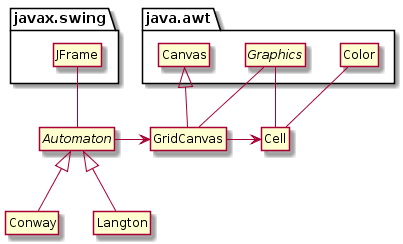
\includegraphics[width=0.75\textwidth,alt={UML class diagram showing inheritance relationships with Automaton as abstract parent class, Conway and Langton as concrete subclasses, GridCanvas extending Canvas, and composition relationships showing how classes contain other objects}]{figs/uml2.png}
\caption{UML class diagram of \java{Conway} and \java{Langton} applications.}
\label{fig:uml2}
\end{center}
\end{figure}

\index{IS-A}
\index{HAS-A}

The diagram shows three examples of inheritance: \java{Conway} is an \java{Automaton}, \java{Langton} is an \java{Automaton}, and \java{GridCanvas} is a \java{Canvas}.
It also shows two examples of composition: \java{Automaton} has a \java{GridCanvas}, and \java{GridCanvas} has a 2D array of \java{Cell}s.

The diagram also shows that \java{Automaton} uses \java{JFrame}, \java{GridCanvas} uses \java{Graphics}, and \java{Cell} uses \java{Graphics} and \java{Color}.

\java{Automaton} is in italics to indicate that it is an abstract class.
As it happens, \java{Graphics} is an abstract class, too.

\index{concrete class}

Conway and Langton are {\bf concrete classes}, because they provide an implementation for all of their methods.
In particular, they implement the \java{update} method that was declared \java{abstract} in \java{Automaton}.

%According to the documentation, its design ``allows an application to draw onto components that are realized on various devices, as well as onto off-screen images.''
%That's the beauty of abstraction; our code works regardless how and where it's drawn.

\index{object-oriented}

One of the challenges of object-oriented programming is keeping track of a large number of classes and the relationships between them.
UML class diagrams can help.


\section{Vocabulary}

\begin{description}

\term{refactor}
To restructure or reorganize existing source code without changing its behavior.

\term{abstract class}
A class that is declared as \java{abstract}; it cannot be instantiated, and it may (or may not) include abstract methods.

\term{concrete class}
A class that is {\em not} declared as \java{abstract}; each of its methods must have an implementation.

\end{description}


\section{Exercises}

The code for this chapter is in the {\it ch16} directory of {\it ThinkJavaCode2}.
See page~\pageref{code} for instructions on how to download the repository.
Before you start the exercises, we recommend that you compile and run the examples.

\begin{exercise}

The last section of this chapter introduced \java{Automaton} as an abstract class and rewrote \java{Conway} as a subclass of \java{Automaton}.
Now it's your turn: rewrite \java{Langton} as a subclass of \java{Automaton}, removing the code that's no longer needed.

\end{exercise}


\begin{exercise}

Mathematically speaking, Game of Life and Langton's Ant are {\em cellular automata}.
``Cellular'' means it has cells, and ``automaton'' means it runs itself.
See \url{https://en.wikipedia.org/wiki/Cellular_automaton} for more discussion.

Implement another cellular automaton of your choice.
You may have to modify \java{Cell} and/or \java{GridCanvas}, in addition to extending \java{Automaton}.
For example, Brian's Brain (\url{https://en.wikipedia.org/wiki/Brian's_Brain}) requires three states: ``on'', ``dying'', and ``off''.

\end{exercise}
